\documentclass[a4paper,12pt]{article}

\usepackage[utf8]{inputenc}
\usepackage[T1]{fontenc}
\usepackage[french]{babel}
\usepackage{geometry}
\geometry{a4paper, margin=2.5cm}
\usepackage{graphicx}
\usepackage{hyperref}

\title{Rapport Projet Planning}
\author{Emad BA GUBAIR, Tom BARTIER, André MARÇAIS, Yann ROBLIN}
\date{\today}

\begin{document}

\maketitle

\tableofcontents
\newpage
\section{Introduction}
Ce document présente le projet PNG (Planning Nouvelle Génération) qui a été réalisé par un groupe d'étudiants
de M1 Maths Info dans le cadre du cours de modéliatione gestion de projet de madame Murisasco, ainsi que 
Jérémy Maloffre et Laurent Loiseau. Le projet consiste à développer une application
de gestion de planning pour une université en Java avec une interface graphique en JavaFX et une base de données
relationnelle. Le groupe a décidé d'utiliser une base de données PostgreSQL ainsi que l'implémentation de JPA Hibernate.
Le projet s'est déroulé sur 4 Sprints d'une semaine et un dernier Sprint de deux semaines pour une équipe de 
4 étudiants.
\section{Présentation des membres du groupe}
Le groupe est composé de 4 membres :\\
Tom Bartier : En charge de la direction du projet ainsi que du bon fonctionnement l'équipe, aussi en charge de la partie
Backend du projet (mise en place de la BD, écriture des classes des objets de la BD, des Repositories pour interagir avec les objets, 
des requêtes JPQL).\\\\
Yann ROBLIN :   \\\\%TODO
Emad BA GUBAIR :   \\\\%TODO
André MARÇAIS :  \\\\%TODO

\section{Glossaire}
\begin{itemize}
    \item Utilisateur : Personne utilisant l'application
    \item Étudiant : Personne suivant des cours
    \item Professeur aussi équivalent à "enseignant" : Personne enseignant des cours
    \item Administrateur : Personne gérant les comptes
    \item Visiteur : Personne non connectée
    \item Secrétaire : Personne gérant les absences
    \item Responsable EDT : Personne gérant l'emploi du temps
    \item Module : Ensemble de cours sur un même thème
    \item Groupe : Ensemble d'étudiants suivant les mêmes cours
    \item Salle : Lieu où se déroulent les cours
    \item Cours aussi équivalent à "créneau" ou "séance" : un cours est un moment réservé dans l'emploi du temps pour un module donné
    \item EDT : Emploi du temps
    \item iCal : Format de fichier pour les calendriers
    \item PDF : Format de fichier pour les documents
    \item Note : Informations supplémentaires sur un cours
    \item Note personnelle : Note ajoutée par un utilisateur sur un cours visible uniquement par lui-même
    \item Note générale : Note ajoutée par un professeur sur un cours visible par tous
\end{itemize}

\section{Expression du besoin et la restitution des interviews}
Identifions les différents types d'utilisateurs de l'application :\\
L'étudiant : Il doit pouvoir consulter son emploi du temps, ses notes personnelles et générales. Il doit également pouvoir ajouter des notes personnelles sur ses cours.\\
Le professeur : Il doit pouvoir consulter son emploi du temps, celui des groupes et des salles, effectuer des demandes d'ajout ou de mofification de cours, 
consulter et modifier les notes générales et sa note personnelle.\\
Le responsable EDT : Il doit pouvoir consulter l'emploi du temps des groupes, des salles et des modules effectuer des demandes 
ajouter et modifier des cours et consulter et accepter ou refuser les différentes demandes des professeurs.\\
Nous avions aussi pensé à d'autres utilisateurs comme le secrétaire qui gère les absences,
l'administrateur qui gère les comptes et le visiteur qui n'est pas connecté, mais nous n'avons pas eu le temps de les implémenter.\\

\section{Exigences}
\subsection{Login}

\begin{itemize}
    \item \textbf{EX\_LOGIN\_001: Créer un compte} \\
    L'administrateur doit pouvoir créer des comptes élève, professeur, et responsable d'emploi du temps.

    \item \textbf{EX\_LOGIN\_002: Se connecter} \\
    L'utilisateur doit pouvoir se connecter qu'il soit élève, professeur ou responsable d'emploi du temps sur une unique interface.

    \item \textbf{EX\_LOGIN\_003: Consulter anonymement} \\
    Les utilisateurs doivent pouvoir accéder anonymement à l'application avec des restrictions.
\end{itemize}

\subsection{Fonctionnalités générales}

\begin{itemize}
    \item \textbf{EX\_BASE\_FEATURES\_001: Consulter emploi du temps personnel} \\
    Les utilisateurs connectés doivent pouvoir consulter leur emploi du temps respectif.

    \item \textbf{EX\_BASE\_FEATURES\_002: Consulter emploi du temps salles} \\
    Les utilisateurs connectés ainsi que les anonymes doivent pouvoir consulter l'emploi du temps des salles.

    \item \textbf{EX\_BASE\_FEATURES\_003: Consulter emploi du temps d'un groupe} \\
    Les utilisateurs connectés doivent pouvoir consulter l'emploi du temps d'un groupe.

    \item \textbf{EX\_BASE\_FEATURES\_004: Consulter emploi du temps d'un professeur} \\
    Les utilisateurs connectés doivent pouvoir consulter l'emploi du temps d'un professeur.

    \item \textbf{EX\_BASE\_FEATURES\_005: Consulter emploi du temps d'un module} \\
    Les utilisateurs connectés doivent pouvoir consulter l'emploi du temps d'un module.

    \item \textbf{EX\_BASE\_FEATURES\_006: Export iCal} \\
    Les utilisateurs connectés doivent pouvoir exporter leur emploi du temps au format iCal.

    \item \textbf{EX\_BASE\_FEATURES\_007: Consulter nombre d'heures par module} \\
    Les utilisateurs peuvent consulter le nombre d'heures d'un module.

    \item \textbf{EX\_BASE\_FEATURES\_008: Consulter le nombre d'heures total} \\
    Les utilisateurs peuvent consulter le nombre d'heures total d'un groupe ou d'un étudiant.

    \item \textbf{EX\_BASE\_FEATURES\_009: Télécharger PDF} \\
    Les utilisateurs peuvent télécharger le planning au format PDF.

    \item \textbf{EX\_BASE\_FEATURES\_010: Rajouter une note sur un cours} \\
    Les professeurs peuvent rajouter une petite note sur un cours.

    \item \textbf{EX\_BASE\_FEATURES\_011: Consulter les notes de cours} \\
    Les étudiants et les professeurs peuvent consulter les petites notes de cours.

    \item \textbf{EX\_BASE\_FEATURES\_012: Création de notes personnelles} \\
    Les notes personnelles sont visibles uniquement par leur auteur. Par exemple, un étudiant peut noter ce qui a été fait ce jour-là si le professeur ne l'a pas noté.
\end{itemize}

\subsection{Report/annulation de cours}

\begin{itemize}
    \item \textbf{EX\_REPORT\_001: Reporter un cours} \\
    Les professeurs doivent pouvoir demander au responsable de l'emploi du temps de reporter un cours.

    \item \textbf{EX\_REPORT\_002: Annuler un cours} \\
    Les professeurs doivent pouvoir demander au responsable de l'emploi du temps d'annuler un cours.

    \item \textbf{EX\_REPORT\_003: Contacter responsable} \\
    Un professeur peut contacter automatiquement le responsable de l'emploi du temps pour réserver une salle à une heure pour un cours.

    \item \textbf{EX\_REPORT\_004: Consulter cours reporté/annulé} \\
    Les utilisateurs connectés peuvent voir la liste des cours reportés ou annulés.
\end{itemize}

\subsection{Absences}

\begin{itemize}
    \item \textbf{EX\_ABSENCES\_001: Faire l'appel} \\
    Les professeurs peuvent faire l'appel pendant un cours.

    \item \textbf{EX\_ABSENCES\_002: Consulter absences sur un cours} \\
    Les professeurs peuvent consulter les élèves qu'ils ont noté comme absents à un cours.

    \item \textbf{EX\_ABSENCES\_003: Étudiant consulter absences} \\
    Les étudiants peuvent consulter leurs absences passées.

    \item \textbf{EX\_ABSENCES\_004: Prévenir d'un retard/absence} \\
    Les étudiants peuvent prévenir les professeurs s'ils ont un retard ou une absence prévue.
\end{itemize}

\subsection{Fonctionnalités Responsable EDT}

\begin{itemize}
    \item \textbf{EX\_RESP\_001: Ajouter un cours} \\
    Le responsable EDT doit pouvoir insérer un nouveau cours avec les informations qui le concernent dans la base de données de l'application. Il peut en définir les droits de modification et copier-coller un cours existant.

    \item \textbf{EX\_RESP\_002: Modifier un cours} \\
    Le responsable EDT doit pouvoir modifier un cours (heure, professeur, module, salle) s'il a les droits de modification sur ce cours.

    \item \textbf{EX\_RESP\_003: Supprimer un cours} \\
    Le responsable EDT doit pouvoir supprimer un cours s'il a les droits de modification sur ce dernier.

    \item \textbf{EX\_RESP\_004: Accepter demande de modification de cours} \\
    Le responsable EDT doit pouvoir accepter une demande de report de cours effectuée par un professeur.

    \item \textbf{EX\_RESP\_005: Reporter un cours} \\
    Le responsable EDT doit pouvoir reporter un cours.

    \item \textbf{EX\_RESP\_006: Annuler un cours} \\
    Le responsable EDT doit pouvoir annuler un cours.
\end{itemize}

\section{Conception UML de l’application}
\begin{figure}[h!]
    \centering
    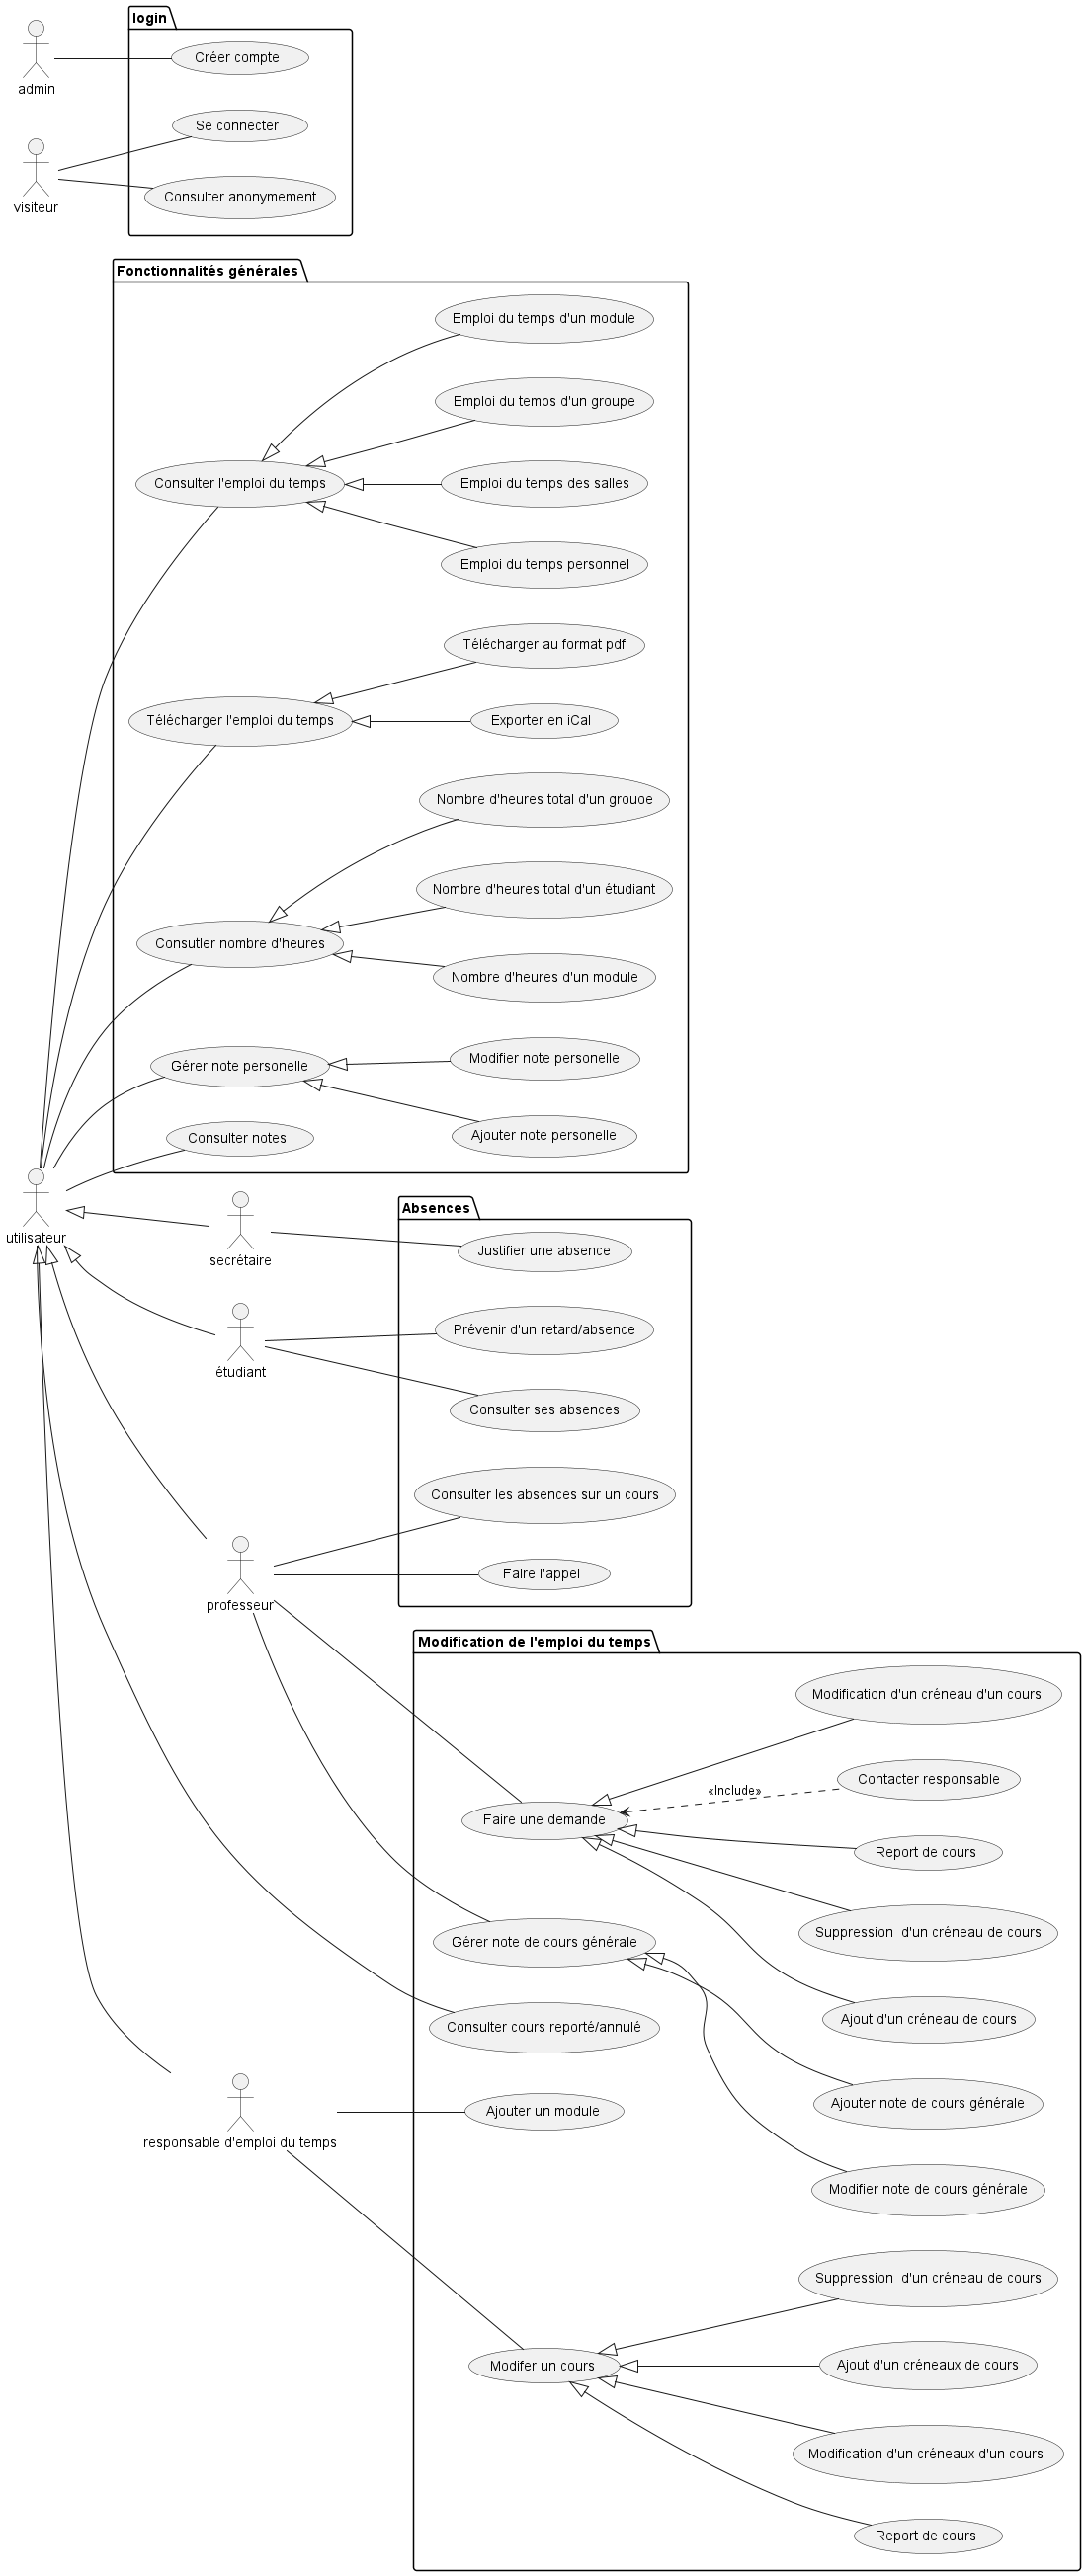
\includegraphics[width=0.65\textwidth]{UC.png}
    \caption{Diagramme de cas d'utilisations}
    \label{fig:uml_diagram}
\end{figure}

\section{La gestion de projet avec le planning, les itérations, la répartition des tâches et le suivi de l’avancement et les difficultés rencontrées}
\section{Le maquettage de l’application}
\section{Le modèle de la base de données}
\section{Les perspectives d’évolution de l’application}

\end{document}